
%% bare_conf.tex
%% V1.4b
%% 2015/08/26
%% by Michael Shell
%% See:
%% http://www.michaelshell.org/
%% for current contact information.
%%
%% This is a skeleton file demonstrating the use of IEEEtran.cls
%% (requires IEEEtran.cls version 1.8b or later) with an IEEE
%% conference paper.
%%
%% Support sites:
%% http://www.michaelshell.org/tex/ieeetran/
%% http://www.ctan.org/pkg/ieeetran
%% and
%% http://www.ieee.org/

%%*************************************************************************
%% Legal Notice:
%% This code is offered as-is without any warranty either expressed or
%% implied; without even the implied warranty of MERCHANTABILITY or
%% FITNESS FOR A PARTICULAR PURPOSE! 
%% User assumes all risk.
%% In no event shall the IEEE or any contributor to this code be liable for
%% any damages or losses, including, but not limited to, incidental,
%% consequential, or any other damages, resulting from the use or misuse
%% of any information contained here.
%%
%% All comments are the opinions of their respective authors and are not
%% necessarily endorsed by the IEEE.
%%
%% This work is distributed under the LaTeX Project Public License (LPPL)
%% ( http://www.latex-project.org/ ) version 1.3, and may be freely used,
%% distributed and modified. A copy of the LPPL, version 1.3, is included
%% in the base LaTeX documentation of all distributions of LaTeX released
%% 2003/12/01 or later.
%% Retain all contribution notices and credits.
%% ** Modified files should be clearly indicated as such, including  **
%% ** renaming them and changing author support contact information. **
%%*************************************************************************


% *** Authors should verify (and, if needed, correct) their LaTeX system  ***
% *** with the testflow diagnostic prior to trusting their LaTeX platform ***
% *** with production work. The IEEE's font choices and paper sizes can   ***
% *** trigger bugs that do not appear when using other class files.       ***                          ***
% The testflow support page is at:
% http://www.michaelshell.org/tex/testflow/



\documentclass[conference]{IEEEtran}
% Some Computer Society conferences also require the compsoc mode option,
% but others use the standard conference format.
%
% If IEEEtran.cls has not been installed into the LaTeX system files,
% manually specify the path to it like:
% \documentclass[conference]{../sty/IEEEtran}





% Some very useful LaTeX packages include:
% (uncomment the ones you want to load)


% *** MISC UTILITY PACKAGES ***
%
%\usepackage{ifpdf}
% Heiko Oberdiek's ifpdf.sty is very useful if you need conditional
% compilation based on whether the output is pdf or dvi.
% usage:
% \ifpdf
%   % pdf code
% \else
%   % dvi code
% \fi
% The latest version of ifpdf.sty can be obtained from:
% http://www.ctan.org/pkg/ifpdf
% Also, note that IEEEtran.cls V1.7 and later provides a builtin
% \ifCLASSINFOpdf conditional that works the same way.
% When switching from latex to pdflatex and vice-versa, the compiler may
% have to be run twice to clear warning/error messages.






% *** CITATION PACKAGES ***
%
%\usepackage{cite}
% cite.sty was written by Donald Arseneau
% V1.6 and later of IEEEtran pre-defines the format of the cite.sty package
% \cite{} output to follow that of the IEEE. Loading the cite package will
% result in citation numbers being automatically sorted and properly
% "compressed/ranged". e.g., [1], [9], [2], [7], [5], [6] without using
% cite.sty will become [1], [2], [5]--[7], [9] using cite.sty. cite.sty's
% \cite will automatically add leading space, if needed. Use cite.sty's
% noadjust option (cite.sty V3.8 and later) if you want to turn this off
% such as if a citation ever needs to be enclosed in parenthesis.
% cite.sty is already installed on most LaTeX systems. Be sure and use
% version 5.0 (2009-03-20) and later if using hyperref.sty.
% The latest version can be obtained at:
% http://www.ctan.org/pkg/cite
% The documentation is contained in the cite.sty file itself.



% *** GRAPHICS RELATED PACKAGES ***
%
\ifCLASSINFOpdf
  \usepackage[pdftex]{graphicx}
  % declare the path(s) where your graphic files are
  % \graphicspath{{../pdf/}{../jpeg/}}
  % and their extensions so you won't have to specify these with
  % every instance of \includegraphics
  % \DeclareGraphicsExtensions{.pdf,.jpeg,.png}
\else
  % or other class option (dvipsone, dvipdf, if not using dvips). graphicx
  % will default to the driver specified in the system graphics.cfg if no
  % driver is specified.
  % \usepackage[dvips]{graphicx}
  % declare the path(s) where your graphic files are
  % \graphicspath{{../eps/}}
  % and their extensions so you won't have to specify these with
  % every instance of \includegraphics
  % \DeclareGraphicsExtensions{.eps}
\fi
% graphicx was written by David Carlisle and Sebastian Rahtz. It is
% required if you want graphics, photos, etc. graphicx.sty is already
% installed on most LaTeX systems. The latest version and documentation
% can be obtained at: 
% http://www.ctan.org/pkg/graphicx
% Another good source of documentation is "Using Imported Graphics in
% LaTeX2e" by Keith Reckdahl which can be found at:
% http://www.ctan.org/pkg/epslatex
%
% latex, and pdflatex in dvi mode, support graphics in encapsulated
% postscript (.eps) format. pdflatex in pdf mode supports graphics
% in .pdf, .jpeg, .png and .mps (metapost) formats. Users should ensure
% that all non-photo figures use a vector format (.eps, .pdf, .mps) and
% not a bitmapped formats (.jpeg, .png). The IEEE frowns on bitmapped formats
% which can result in "jaggedy"/blurry rendering of lines and letters as
% well as large increases in file sizes.
%
% You can find documentation about the pdfTeX application at:
% http://www.tug.org/applications/pdftex





% *** MATH PACKAGES ***
%
%\usepackage{amsmath}
% A popular package from the American Mathematical Society that provides
% many useful and powerful commands for dealing with mathematics.
%
% Note that the amsmath package sets \interdisplaylinepenalty to 10000
% thus preventing page breaks from occurring within multiline equations. Use:
%\interdisplaylinepenalty=2500
% after loading amsmath to restore such page breaks as IEEEtran.cls normally
% does. amsmath.sty is already installed on most LaTeX systems. The latest
% version and documentation can be obtained at:
% http://www.ctan.org/pkg/amsmath





% *** SPECIALIZED LIST PACKAGES ***
%
%\usepackage{algorithmic}
% algorithmic.sty was written by Peter Williams and Rogerio Brito.
% This package provides an algorithmic environment fo describing algorithms.
% You can use the algorithmic environment in-text or within a figure
% environment to provide for a floating algorithm. Do NOT use the algorithm
% floating environment provided by algorithm.sty (by the same authors) or
% algorithm2e.sty (by Christophe Fiorio) as the IEEE does not use dedicated
% algorithm float types and packages that provide these will not provide
% correct IEEE style captions. The latest version and documentation of
% algorithmic.sty can be obtained at:
% http://www.ctan.org/pkg/algorithms
% Also of interest may be the (relatively newer and more customizable)
% algorithmicx.sty package by Szasz Janos:
% http://www.ctan.org/pkg/algorithmicx




% *** ALIGNMENT PACKAGES ***
%
%\usepackage{array}
% Frank Mittelbach's and David Carlisle's array.sty patches and improves
% the standard LaTeX2e array and tabular environments to provide better
% appearance and additional user controls. As the default LaTeX2e table
% generation code is lacking to the point of almost being broken with
% respect to the quality of the end results, all users are strongly
% advised to use an enhanced (at the very least that provided by array.sty)
% set of table tools. array.sty is already installed on most systems. The
% latest version and documentation can be obtained at:
% http://www.ctan.org/pkg/array


% IEEEtran contains the IEEEeqnarray family of commands that can be used to
% generate multiline equations as well as matrices, tables, etc., of high
% quality.




% *** SUBFIGURE PACKAGES ***
%\ifCLASSOPTIONcompsoc
%  \usepackage[caption=false,font=normalsize,labelfont=sf,textfont=sf]{subfig}
%\else
%  \usepackage[caption=false,font=footnotesize]{subfig}
%\fi
% subfig.sty, written by Steven Douglas Cochran, is the modern replacement
% for subfigure.sty, the latter of which is no longer maintained and is
% incompatible with some LaTeX packages including fixltx2e. However,
% subfig.sty requires and automatically loads Axel Sommerfeldt's caption.sty
% which will override IEEEtran.cls' handling of captions and this will result
% in non-IEEE style figure/table captions. To prevent this problem, be sure
% and invoke subfig.sty's "caption=false" package option (available since
% subfig.sty version 1.3, 2005/06/28) as this is will preserve IEEEtran.cls
% handling of captions.
% Note that the Computer Society format requires a larger sans serif font
% than the serif footnote size font used in traditional IEEE formatting
% and thus the need to invoke different subfig.sty package options depending
% on whether compsoc mode has been enabled.
%
% The latest version and documentation of subfig.sty can be obtained at:
% http://www.ctan.org/pkg/subfig




% *** FLOAT PACKAGES ***
%
%\usepackage{fixltx2e}
% fixltx2e, the successor to the earlier fix2col.sty, was written by
% Frank Mittelbach and David Carlisle. This package corrects a few problems
% in the LaTeX2e kernel, the most notable of which is that in current
% LaTeX2e releases, the ordering of single and double column floats is not
% guaranteed to be preserved. Thus, an unpatched LaTeX2e can allow a
% single column figure to be placed prior to an earlier double column
% figure.
% Be aware that LaTeX2e kernels dated 2015 and later have fixltx2e.sty's
% corrections already built into the system in which case a warning will
% be issued if an attempt is made to load fixltx2e.sty as it is no longer
% needed.
% The latest version and documentation can be found at:
% http://www.ctan.org/pkg/fixltx2e


%\usepackage{stfloats}
% stfloats.sty was written by Sigitas Tolusis. This package gives LaTeX2e
% the ability to do double column floats at the bottom of the page as well
% as the top. (e.g., "\begin{figure*}[!b]" is not normally possible in
% LaTeX2e). It also provides a command:
%\fnbelowfloat
% to enable the placement of footnotes below bottom floats (the standard
% LaTeX2e kernel puts them above bottom floats). This is an invasive package
% which rewrites many portions of the LaTeX2e float routines. It may not work
% with other packages that modify the LaTeX2e float routines. The latest
% version and documentation can be obtained at:
% http://www.ctan.org/pkg/stfloats
% Do not use the stfloats baselinefloat ability as the IEEE does not allow
% \baselineskip to stretch. Authors submitting work to the IEEE should note
% that the IEEE rarely uses double column equations and that authors should try
% to avoid such use. Do not be tempted to use the cuted.sty or midfloat.sty
% packages (also by Sigitas Tolusis) as the IEEE does not format its papers in
% such ways.
% Do not attempt to use stfloats with fixltx2e as they are incompatible.
% Instead, use Morten Hogholm'a dblfloatfix which combines the features
% of both fixltx2e and stfloats:
%
% \usepackage{dblfloatfix}
% The latest version can be found at:
% http://www.ctan.org/pkg/dblfloatfix




% *** PDF, URL AND HYPERLINK PACKAGES ***
%
%\usepackage{url}
% url.sty was written by Donald Arseneau. It provides better support for
% handling and breaking URLs. url.sty is already installed on most LaTeX
% systems. The latest version and documentation can be obtained at:
% http://www.ctan.org/pkg/url
% Basically, \url{my_url_here}.




% *** Do not adjust lengths that control margins, column widths, etc. ***
% *** Do not use packages that alter fonts (such as pslatex).         ***
% There should be no need to do such things with IEEEtran.cls V1.6 and later.
% (Unless specifically asked to do so by the journal or conference you plan
% to submit to, of course. )


% correct bad hyphenation here
\hyphenation{op-tical net-works semi-conduc-tor}


\begin{document}
%
% paper title
% Titles are generally capitalized except for words such as a, an, and, as,
% at, but, by, for, in, nor, of, on, or, the, to and up, which are usually
% not capitalized unless they are the first or last word of the title.
% Linebreaks \\ can be used within to get better formatting as desired.
% Do not put math or special symbols in the title.
\title{An Investigation of Multiple Language Classifiers \\COMP 551 - Applied Machine Learning}


% author names and affiliations
% use a multiple column layout for up to three different
% affiliations
\author{\IEEEauthorblockN{Thomas Page}
\IEEEauthorblockA{Department of Mechanical Engineering\\
McGill University\\
Montreal, Canada\\
thomas.page@mail.mcgill.ca\\
260771672}
\and
\IEEEauthorblockN{David Tamrazov}
\IEEEauthorblockA{Computer Science, Arts\\
McGill University\\
Montreal, Canada\\
david.tamrazov@mail.mcgill.ca\\
260561439}
\and
\IEEEauthorblockN{Alexander Wong}
\IEEEauthorblockA{Cognitive Science, Arts and Science\\
McGill University\\
Montreal, Canada\\
alexander.wong4@mail.mcgill.ca\\
260602944}}


% make the title area
\maketitle
\begin{flushleft}
Notorious Language Classifiers\\
https://github.com/a22wong/notorious-language-classifier\\
\end{flushleft}

\hfill October 23, 2017

% For peer review papers, you can put extra information on the cover
% page as needed:
% \ifCLASSOPTIONpeerreview
% \begin{center} \bfseries EDICS Category: 3-BBND \end{center}
% \fi
%
% For peerreview papers, this IEEEtran command inserts a page break and
% creates the second title. It will be ignored for other modes.
\IEEEpeerreviewmaketitle



\section{Introduction}
As a result of the first project, corpora in various languages are available to act as training sets for many language related machine learning tasks. The goal of this project is to create classifiers that can determine the language of a sample of text from corpora information developed in the first project. Based on a review of the methods discussed in COMP 551, we construct four classifiers: Naive Bayes, Linear Discriminant Analysis (LDA), Decision Trees, and Extremely Randomized Decision Trees.


\section{Related Work}
Naive Bayes was chosen as the most promising text classification method for this application based on a previous study in this area. In his master’s thesis, Jason Rennie used a Naive Bayes classifier to classify a given news article into 1 of 20 different categories (e.g. Electronics, Religion, Space, etc.). Training on 1000 documents from each category, the Naive Bayes classifier was able to classify the new articles very well ~\cite{Rennie}. The main difference between that task and this project is that rather than distinguishing between categories, we will be distinguishing between languages, but the same concept applies. 


\section{Problem Representation}
The compiled training dataset contains 276516 labeled language samples from five different languages: Slovak, French, Spanish, German, and Polish. The test set contains 118507 unlabeled samples of zero to ten individual characters. This presented the challenge of classifying seemingly nonsensical data; a common task in practical machine learning. Fig.~\ref{class_distribution} represents the weight of each language in the training set. 

We found that the data required little pre-processing as non-discriminative symbols such as punctuation had already been removed. To process the text, we chose to simply make all characters lowercase as to eliminate the classifier distinguishing between upper- and lower-case symbols. There are many blank lines in the training set, but we found eliminating them to have no effect on our outcome. Nothing is being assigned to a label in these blank lines, and therefore it does not add any weight to the prediction. We also looked into removing numbers from our training set as these have no attachment to language. However, as the corpora are taken from different sources, we decided that some sources may be more likely to include numbers in the dialogue and that we could exploit this distinction.

\subsection{Naive Bayes}
As mentioned, the test set is a string of characters. Because of this, we chose to train our classifiers on the probability of characters appearing rather than the probability of words or small groups of words appearing. We lost a lot of the natural language data by making our features individual characters, but this seemed to be the only reasonable solution for this unique problem. 

\subsection{Decision Tree}
With a 'unexpected' test set of only single characters, we decided to try using a Decision Tree to discriminate test data based on what special characters appeared, and default to a Naive Bayes approach when no special characters appeared. Initial data pre-processing required included identifying all special characters, which we did so by regular expression matching any non-ASCII character. We found there to be 613 non-ASCII characters present in the training set; later this will shown to be too large to use for classification in limited processing time.

Next was to classify the special characters to the language they were unique to. Special characters that mapped to more than one language were not used in the Decision Tree evaluation criteria. However, due to failure to properly implement a program that properly identified special characters, we were unable to implement a Decision Tree algorithm 

The initial set of 613 special characters was far too large, reporting over 200 special characters unique to French alone. Attempting to implement the Decision Tree with this set of characters has a time complexity of \texttt{O(shcn)} where \texttt{s} is the number of special characters unique to the language being filtered at level \texttt{h} of the Decision Tree, for each character \texttt{c} in each test case \texttt{n}. On a commercial computer, it was making ~3 predictions a second, which would have required over a full day of computation.

We tried to streamline the data pre-processing to find a better method without sucess. Specifically, the encountered issue was with unicode encoding, and we suspect specifically with 8 vs 16 bit encoding for special characters that, in the given dataset, actually are two chars in line; for example, the character \texttt{\`{a}} is given by the unicode sequence \texttt{0xc3} and \texttt{0xa0}.

In designing the Decision Tree, the goal was to have each node's evaluation criteria make the largest cut in the test set - in other words create the most separation - to effectively filter the test data. So, assuming the training and test sets would have similar distributions of classes, we structured the tree to evaluate most likely languages first: French, Spanish, German, Polish, then Slovak.


\begin{figure}[htbp]
\centering
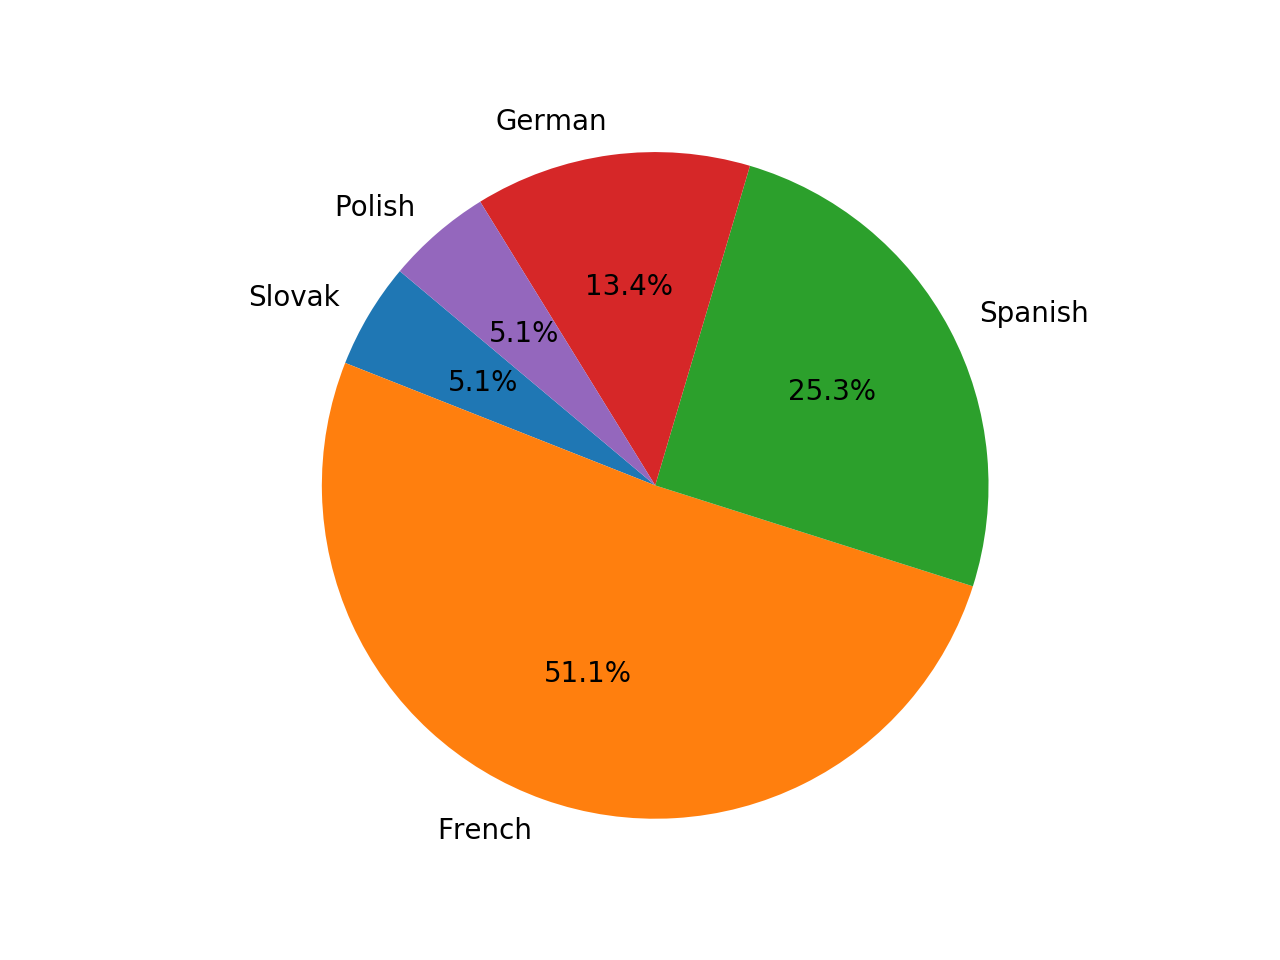
\includegraphics[width=70mm]{class_distribution.png}
\caption{Training set language distribution.}
\label{class_distribution}
\end{figure}


\section{Testing and Validation}
The most effective way to represent the performance metrics of each individual classifier is through their respective confusion matrix. We chose to evaluate our classifiers using a normalized confusion matrix as it highlights important outputs like the true positives and exactly how each class is correctly or incorrectly classified.

\subsection{Naive Bayes}
Fig.~\ref{confusion_bayes} shows the confusion matrix for the Naive Bayes classifier on the training set. Slovak, French, German, and Polish are all classified 90\% correctly. Spanish is the only classifier with a significant difference at 77\% correct. It is clear from the matrix that most of the incorrect Spanish classifications are classified at French. This is due in part to both languages sharing many of the same symbols, and because French accounts for over double the training set samples, a Spanish sample is more likely to be classified as French than vice versa. This hypothesis is supported by the confusion matrix, as 16\% of Spanish samples are classified as French, but only 7\% of French samples are classified as Spanish.

\begin{figure}[htbp]
\centering
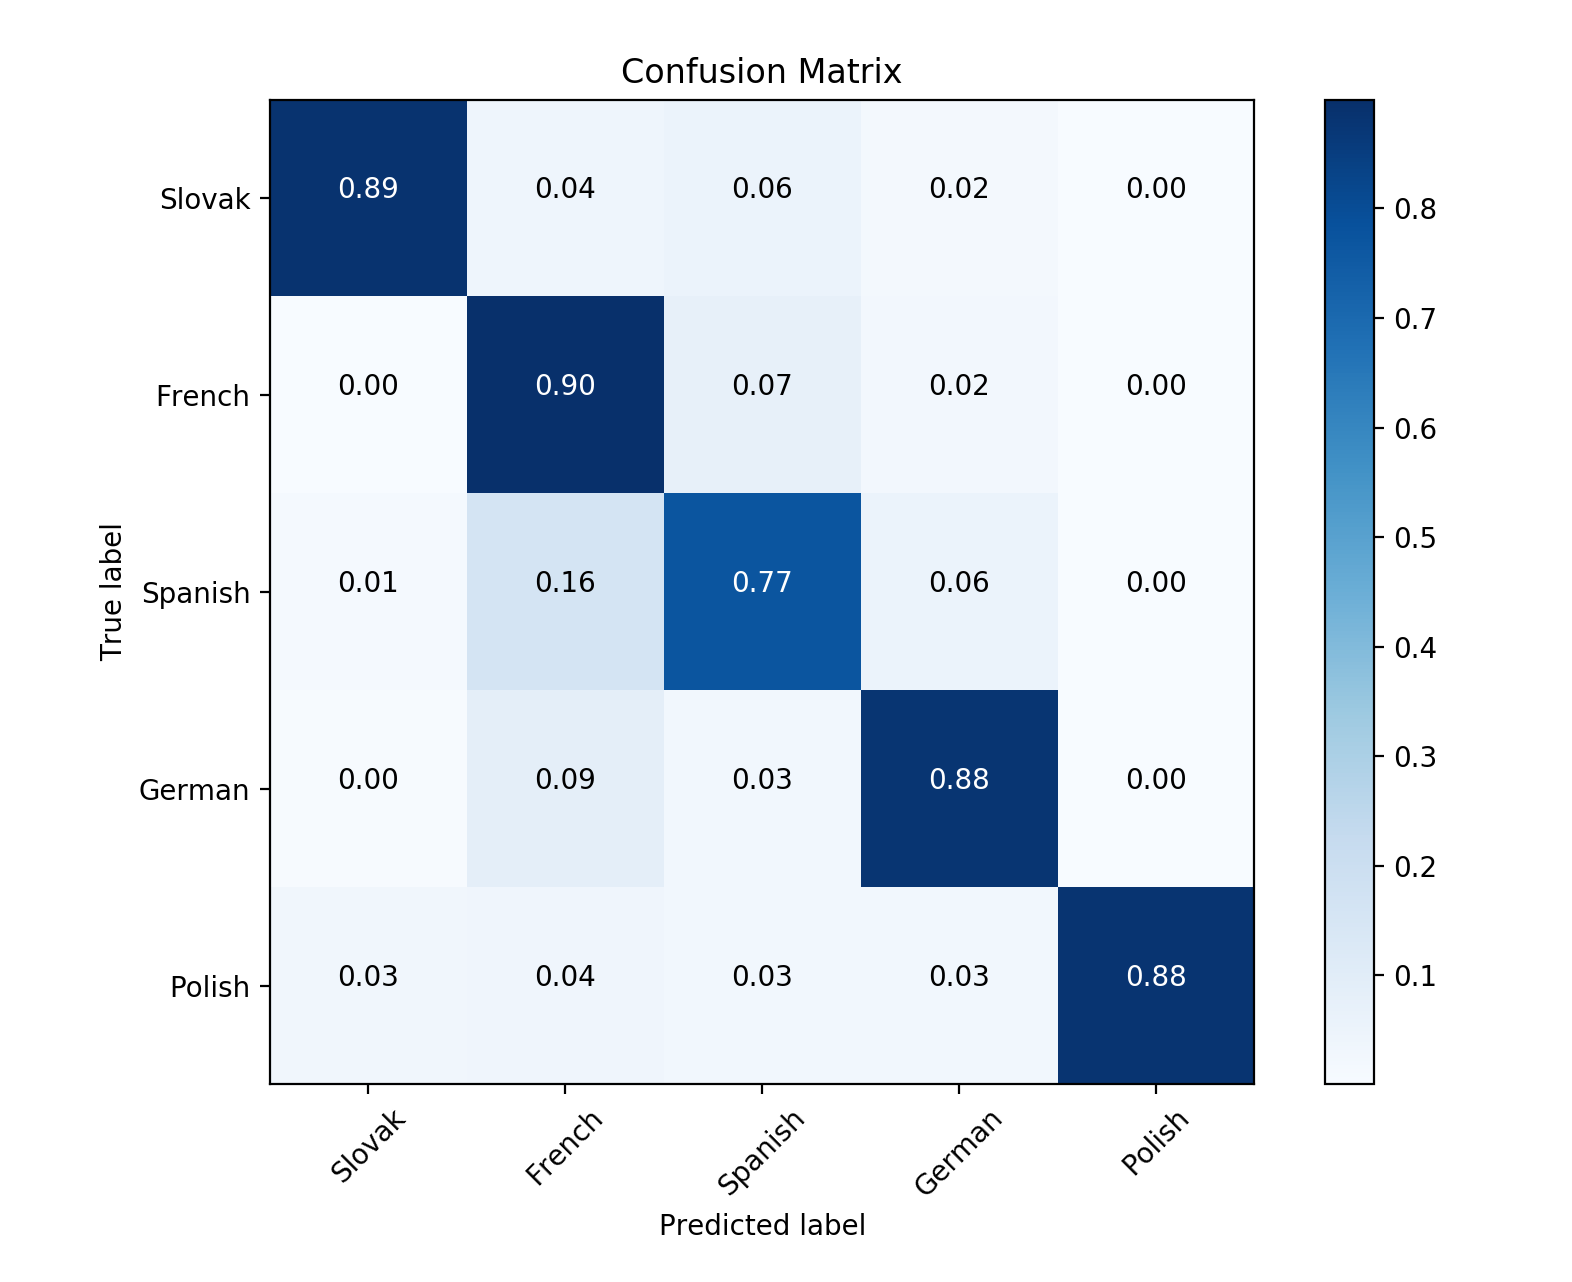
\includegraphics[width=80mm]{confusion_bayes.png}
\caption{Naive Bayes confusion matrix.}
\label{confusion_bayes}
\end{figure}

\subsection{Decision Tree}
The expected outcome was that of higher accuracy than Naive Bayes, as it essentially filters out test cases with special characters unique to their respective language. However, due to the special character decoding problem mentioned prior, we were unable to fully test the potential of this method.

For proof of concept, we did implement an incomplete method that lacked sufficient pre-processing of special characters, but out of the 118507 test cases, the Decision Tree only made a decision 148 times - insignificant. Thus, the test accuracy and consequently the confusion matrix for the Decision Tree implementation is the same as that of Naive Bayes in Fig.~\ref{confusion_bayes} above.



\subsection{Extremely Randomized Trees}


\section{Discussion}
\subsection{Naive Bayes}
Several attempts were made at achieving a higher score using the Naive Bayes classifier. The lower true positive rate of the Spanish classifications were of concern. To remedy this, a corpus of ~100,000 Spanish words was added to the training set. This did improve the Spanish rate, but lowered the French rate and overall accuracy of the classifier. In another attempt, a French corpus was added in conjunction with the Spanish corpus, but this led to a very similar result to the initial classifier.
The log-likelihood was also calculated in an attempt to improve the classification score, but again there was little difference in the actual output at the expense of a much more complex calculation. Ultimately, the basic Naive Bayes seemed to perform best. Future work in this area will involve testing a Naive Bayes classifier available in a library like sklearn to see how the results compare to the one developed from scratch here. 

\subsection{Decision Tree}
Dealing with the encoding issues revealed many possible hurdles in pre-processing the data, and for evaluating the Decision Tree algorithm. If we had been able to properly decode the special characters, we might have been able to do better diagnostics to create a near-optimal tree structure, rather than the reality of implementing a pre-Naive Bayes filter.

Because the planned implementation was to immediately filter a test case if it contained a character that mapped uniquely to one class, the Decision Tree would be extremely susceptible to errors in test set. Redundancies could have been included, such as by predicting the \texttt{argmax} of classes of special characters appearing in a test case.

Though special characters that mapped to more than one language were not used in the Decision Tree evaluation criteria, they could be utilized in a more robust, probabilistic method that used the  Bayesian probabilities calculated from special character sets alone, instead of just the training set.

Ultimately, even if the Decision Tree method was more effective, it is essentially a data pre-processing step prior to Naive Bayes. 


\subsection{Extremely Randomized Trees}
\subsection{Linear Discriminant Analysis} %% if you want to write about this David, i.e what went wrong with it


\section{Statement of Contributions}
Thomas was responsible for fully implementing the Naive Bayes classifier. He also wrote the Introduction, Related Work, and Problem Representation sections of the report as well as any sections pertaining to Naive Bayes.

Alex was responsible for fully implementing the Decision Trees classifier. For the report, he wrote any sections pertaining to Decision Trees.

David was responsible for the LDA and Extremely Randomized Trees classifiers. For the report, he wrote any sections pertaining to LDA or Extremely Randomized Trees.

We hereby state that all the work presented in this report is that of the authors.



% Note that the IEEE typically puts floats only at the top, even when this
% results in a large percentage of a column being occupied by floats.


% An example of a double column floating figure using two subfigures.
% (The subfig.sty package must be loaded for this to work.)
% The subfigure \label commands are set within each subfloat command,
% and the \label for the overall figure must come after \caption.
% \hfil is used as a separator to get equal spacing.
% Watch out that the combined width of all the subfigures on a 
% line do not exceed the text width or a line break will occur.
%
%\begin{figure*}[!t]
%\centering
%\subfloat[Case I]{\includegraphics[width=2.5in]{box}%
%\label{fig_first_case}}
%\hfil
%\subfloat[Case II]{\includegraphics[width=2.5in]{box}%
%\label{fig_second_case}}
%\caption{Simulation results for the network.}
%\label{fig_sim}
%\end{figure*}
%
% Note that often IEEE papers with subfigures do not employ subfigure
% captions (using the optional argument to \subfloat[]), but instead will
% reference/describe all of them (a), (b), etc., within the main caption.
% Be aware that for subfig.sty to generate the (a), (b), etc., subfigure
% labels, the optional argument to \subfloat must be present. If a
% subcaption is not desired, just leave its contents blank,
% e.g., \subfloat[].


% An example of a floating table. Note that, for IEEE style tables, the
% \caption command should come BEFORE the table and, given that table
% captions serve much like titles, are usually capitalized except for words
% such as a, an, and, as, at, but, by, for, in, nor, of, on, or, the, to
% and up, which are usually not capitalized unless they are the first or
% last word of the caption. Table text will default to \footnotesize as
% the IEEE normally uses this smaller font for tables.
% The \label must come after \caption as always.
%
%\begin{table}[!t]
%% increase table row spacing, adjust to taste
%\renewcommand{\arraystretch}{1.3}
% if using array.sty, it might be a good idea to tweak the value of
% \extrarowheight as needed to properly center the text within the cells
%\caption{An Example of a Table}
%\label{table_example}
%\centering
%% Some packages, such as MDW tools, offer better commands for making tables
%% than the plain LaTeX2e tabular which is used here.
%\begin{tabular}{|c||c|}
%\hline
%One & Two\\
%\hline
%Three & Four\\
%\hline
%\end{tabular}
%\end{table}


% trigger a \newpage just before the given reference
% number - used to balance the columns on the last page
% adjust value as needed - may need to be readjusted if
% the document is modified later
%\IEEEtriggeratref{8}
% The "triggered" command can be changed if desired:
%\IEEEtriggercmd{\enlargethispage{-5in}}

% references section

% can use a bibliography generated by BibTeX as a .bbl file
% BibTeX documentation can be easily obtained at:
% http://mirror.ctan.org/biblio/bibtex/contrib/doc/
% The IEEEtran BibTeX style support page is at:
% http://www.michaelshell.org/tex/ieeetran/bibtex/
%\bibliographystyle{IEEEtran}
% argument is your BibTeX string definitions and bibliography database(s)
%\bibliography{IEEEabrv,../bib/paper}
%
% <OR> manually copy in the resultant .bbl file
% set second argument of \begin to the number of references
% (used to reserve space for the reference number labels box)
\begin{thebibliography}{1}

\bibitem{Rennie}
J. D. M. Rennie, ``Improving Multi-class Text Classification with Naive Bayes,'' M.S. thesis, Department of Electrical Engineering and Computer Science, Massachusetts Institute of Technology, Cambridge, Massachusetts, 2001. 

\end{thebibliography}




% that's all folks
\end{document}


